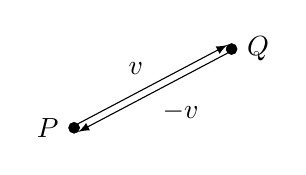
\begin{tikzpicture}[
	point/.style={circle,draw,very thin,fill,inner sep=0pt,minimum size=4pt},
	vector/.style={-latex},
]
	\node[point] at (0,0) (p) [label=left:{$P$}] {};
	\node[point] at (2,1) (q) [label=right:{$Q$}] {};
	\draw[vector] (p.north east) to node[above left] {$\uvec{v}$} (q.north west);
	\draw[vector] (q.south west) to node[below right] {$-\uvec{v}$} (p.south east);
\end{tikzpicture}
